\chapter{Конструкторская часть}

В данной части будут разработаны функциональные схемы разрабатываемого ПО, а также разработаны структуры и алгоритмы, которые будут использованы в ПО.

\section{Функциональные схемы} 

На рисунках \ref{fig:A0} -- \ref{fig:A3} представлено формальное описании разрабатываемого ПО в виде idef0-диаграммы.

\begin{figure}[H]
	\centering
	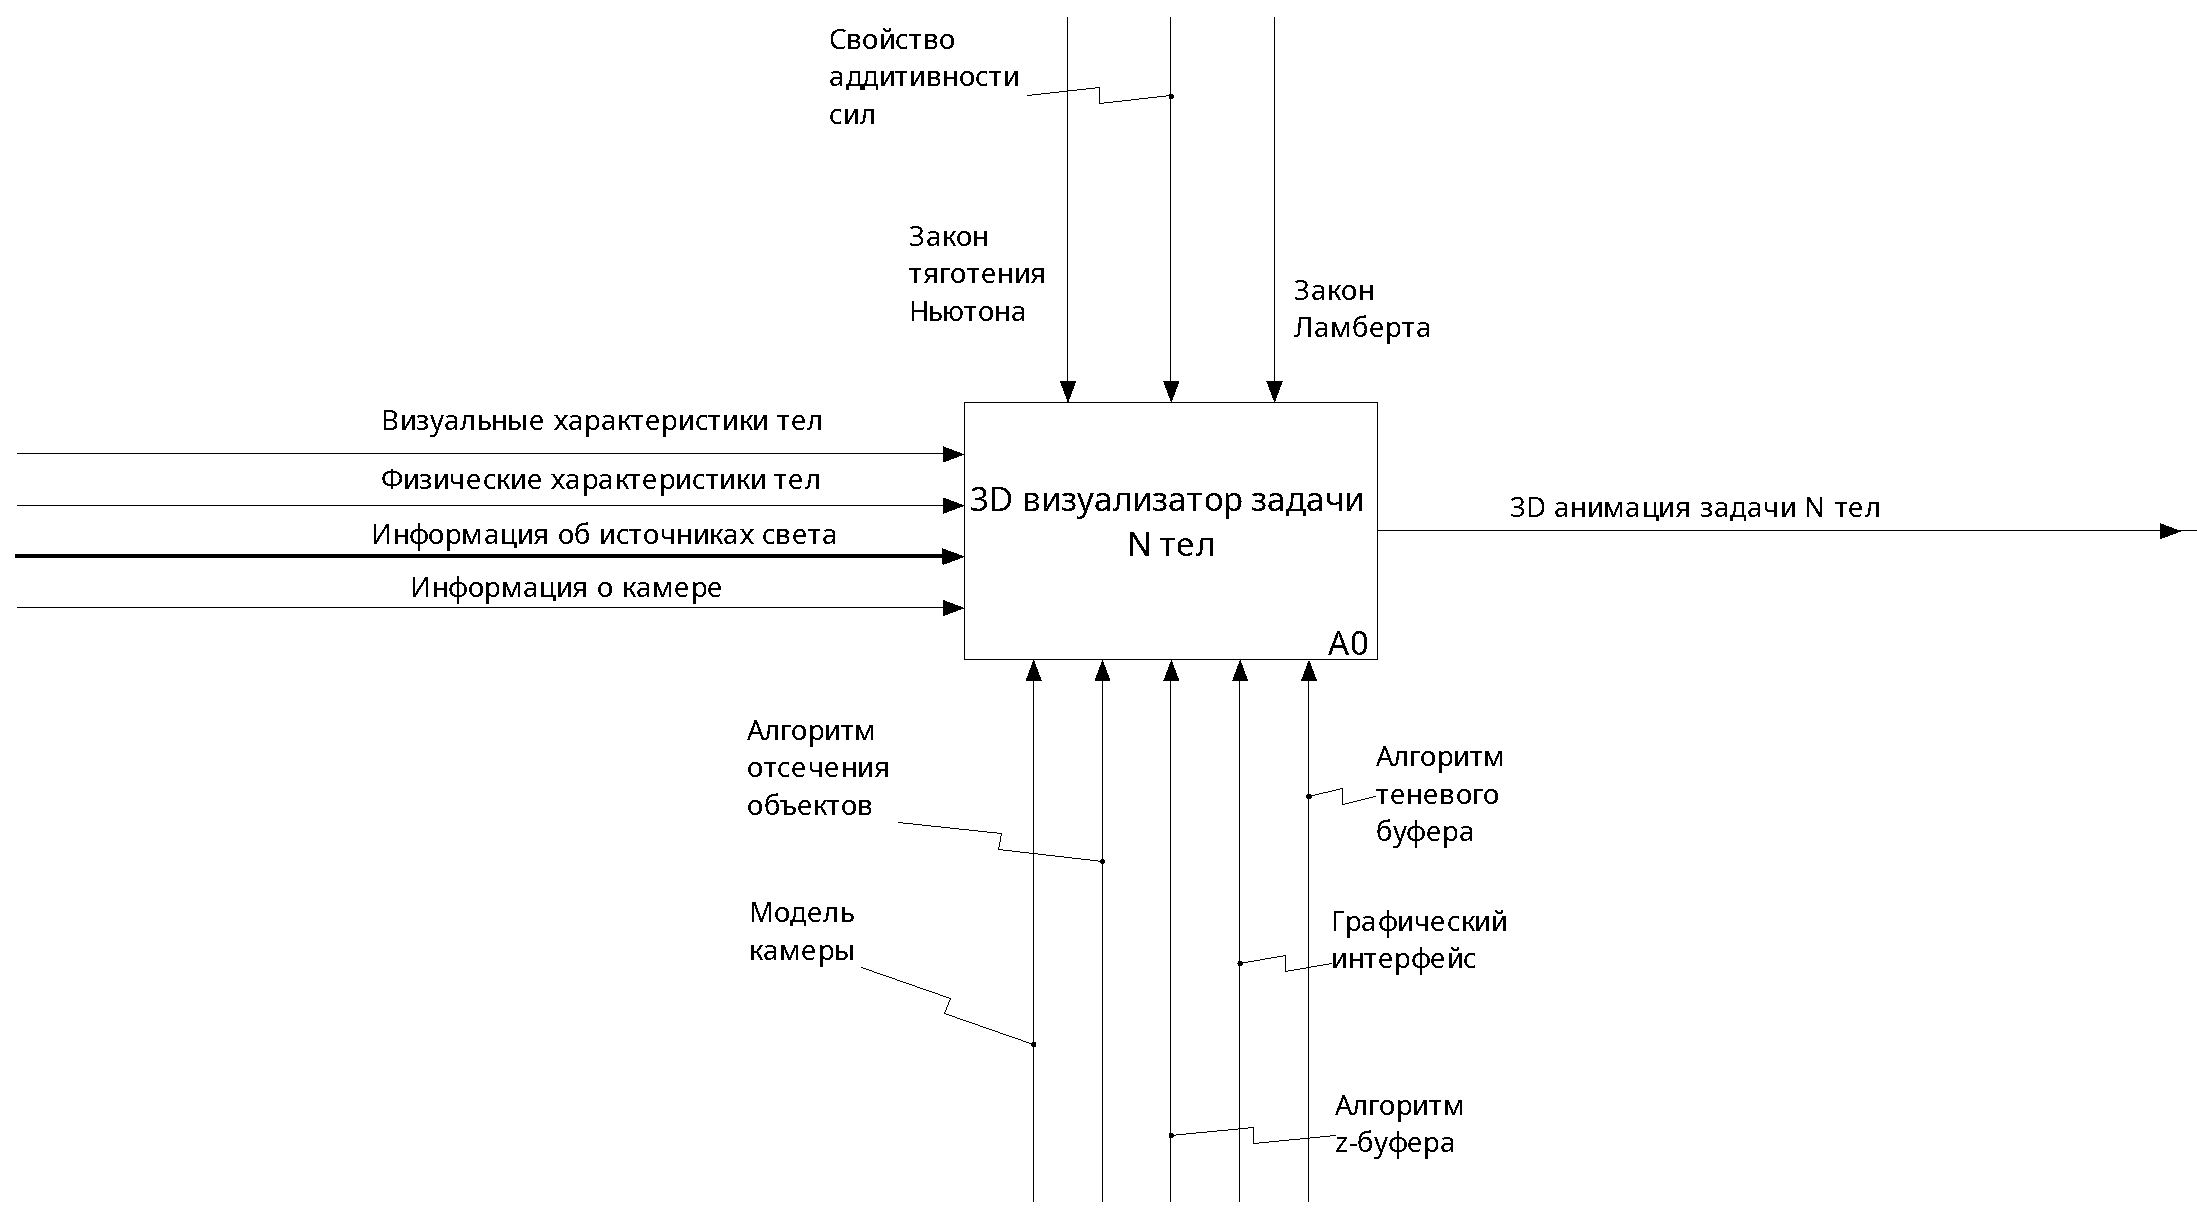
\includegraphics[width=0.9\textwidth]{ramus/01_A0}
	\caption{"Контекстная диаграмма верхнего уровня"}
	\label{fig:A0}
\end{figure}

\begin{figure}[H]
	\centering
	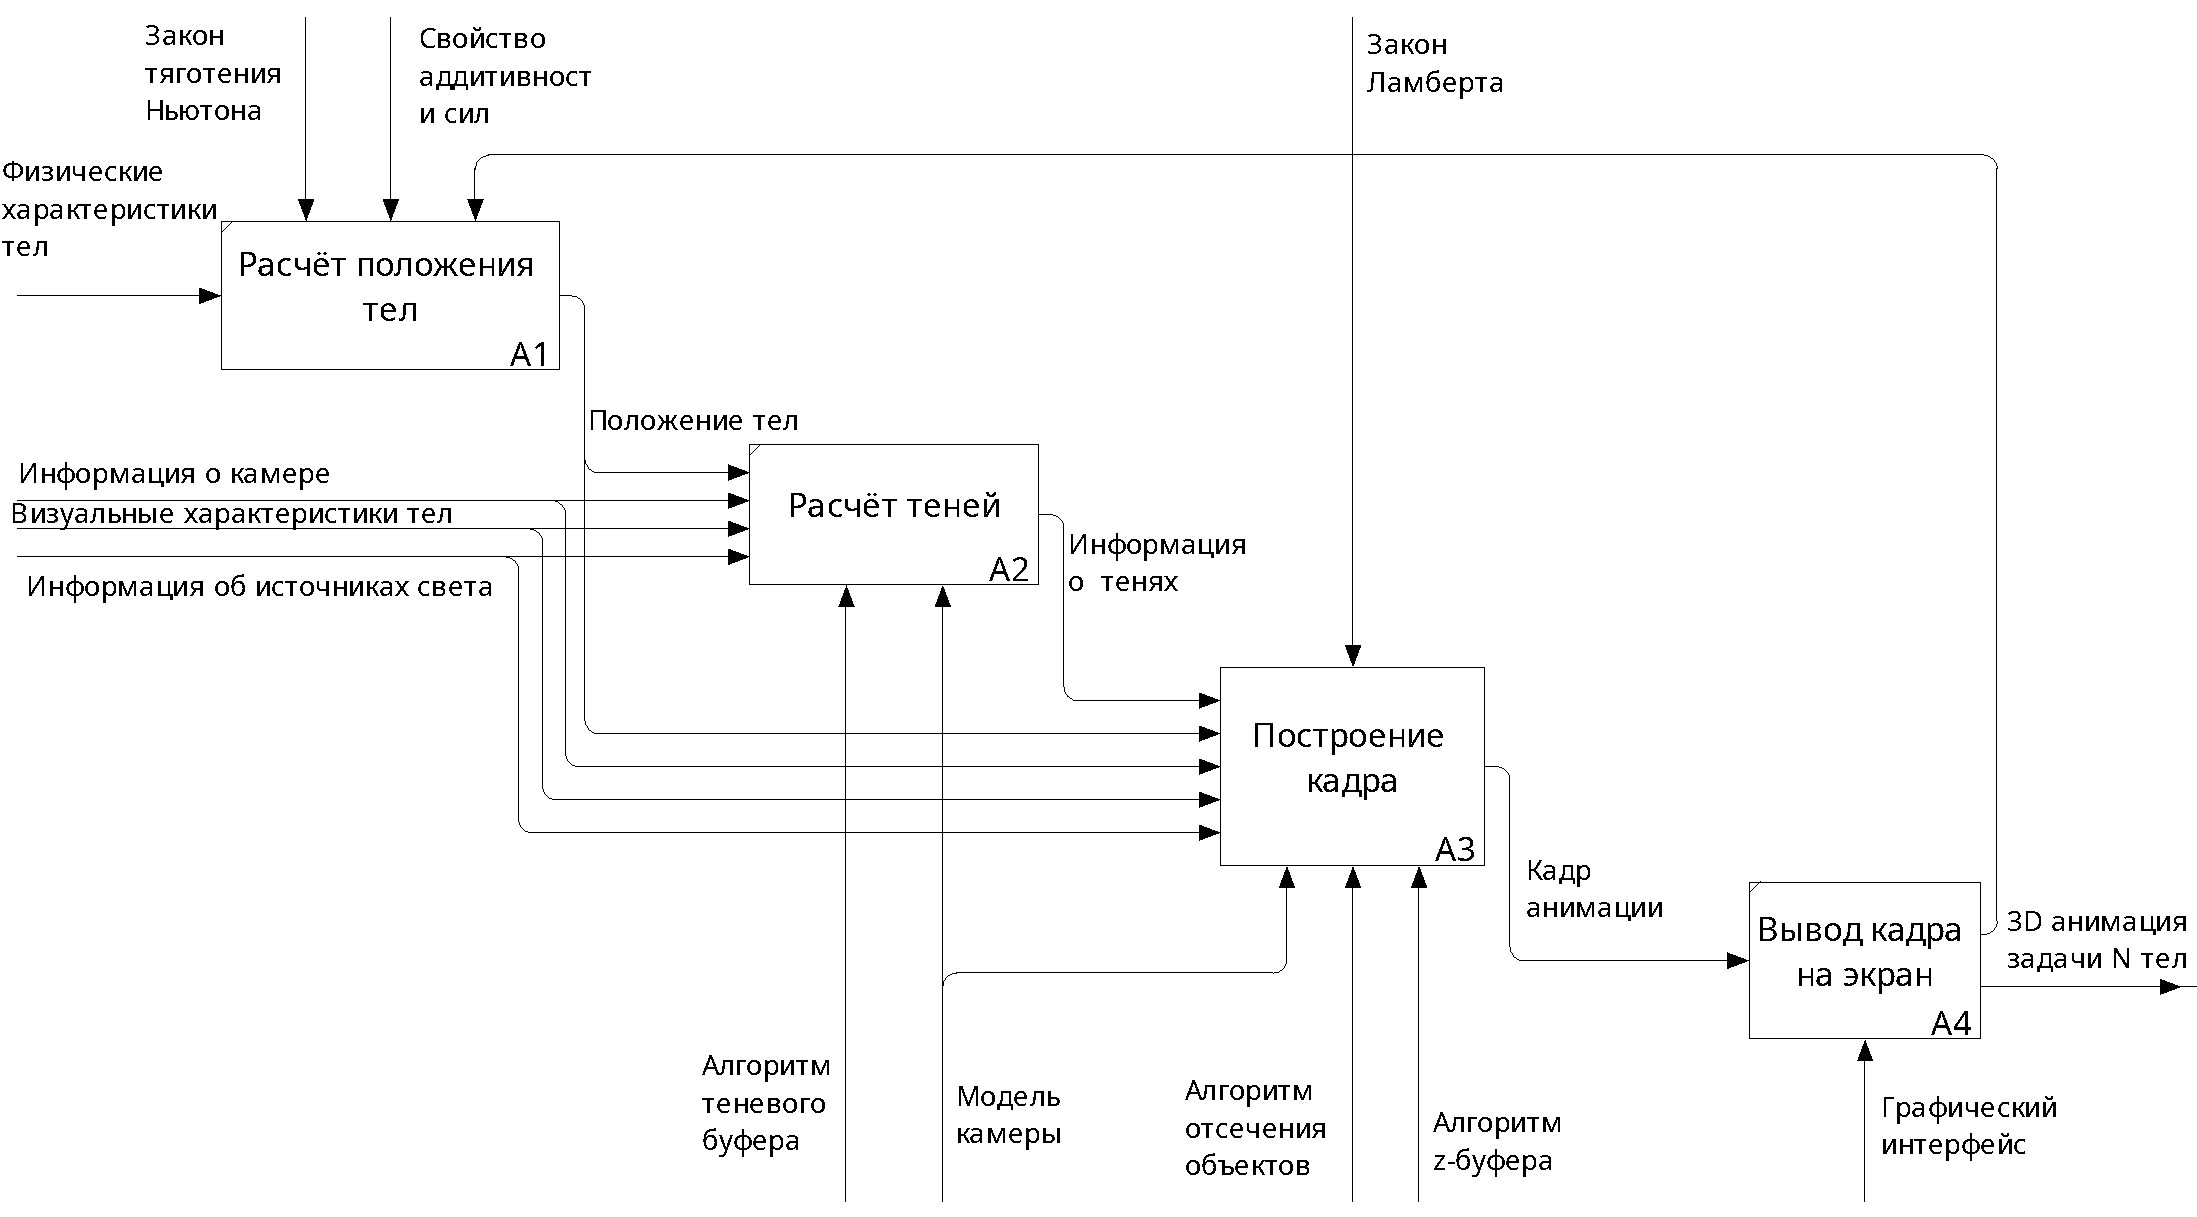
\includegraphics[width=0.9\textwidth]{ramus/02_A0}
	\caption{"Основной цикл ПО"}
	\label{fig:A1}
\end{figure}

\begin{figure}[H]
	\centering
	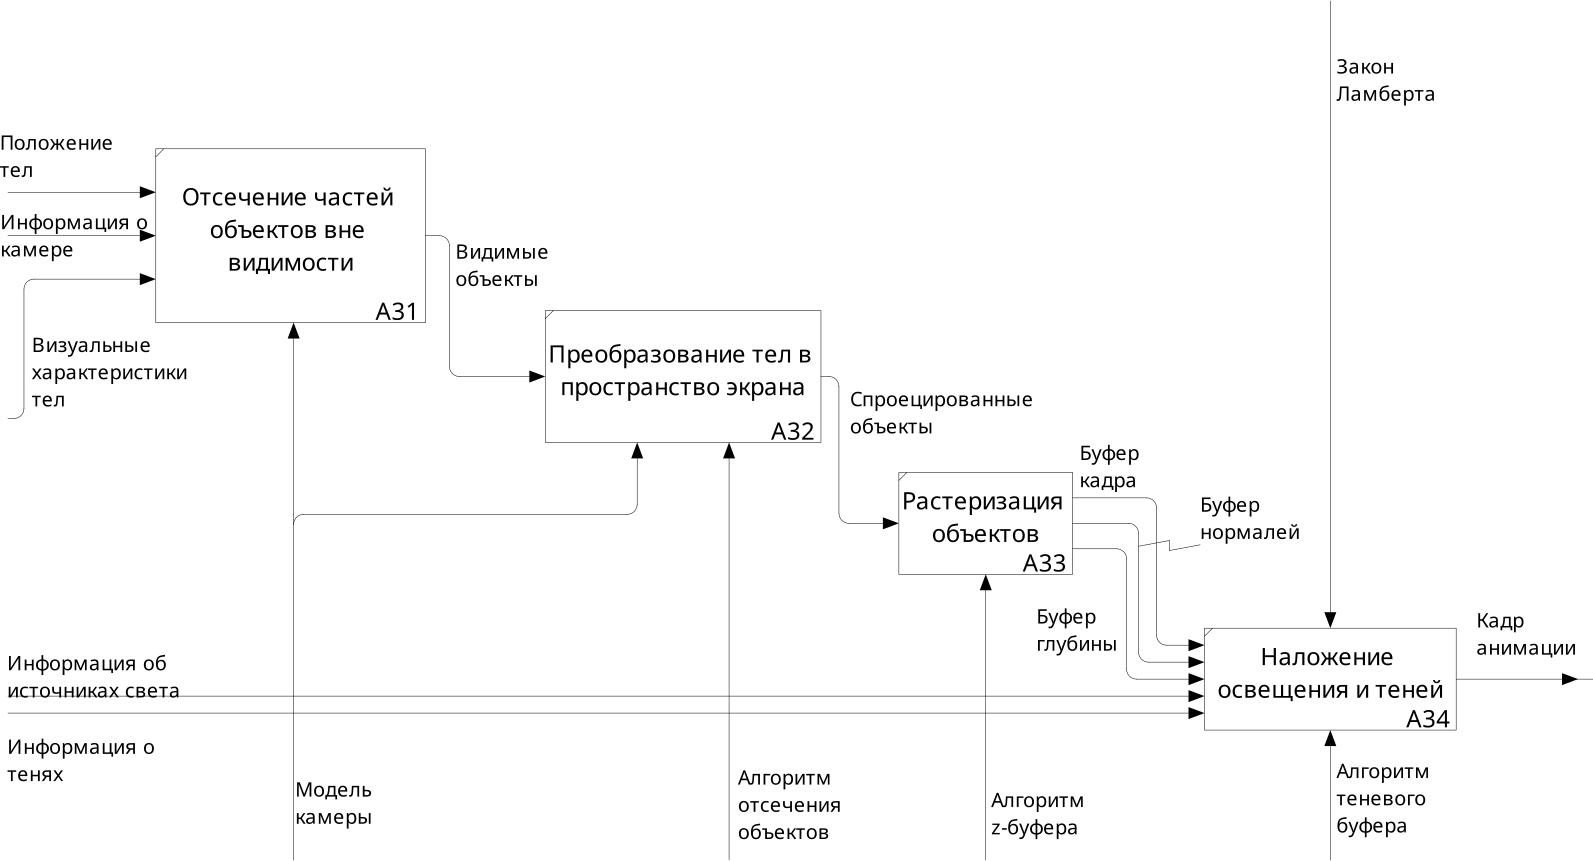
\includegraphics[width=0.9\textwidth]{ramus/03_A3}
	\caption{"Построение кадра"}
	\label{fig:A3}
\end{figure}




\section*{Вывод}

\clearpage
